\section{Proposed Method}
\label{sec:proposed-method}

The proposed method utilizes meteorological forecast data such as forecast cloudiness or forecast irradiance to forecast the PV system output for the upcoming 12 to 72 hours, which called the ``day-ahead forecast''.
It is assumed that these meteorological forecasts will be updated once or at most a few times per day.
Throughout the day, the current day's PV output forecast is updated by applying one of several available time-series forecasting techniques.
A high-level diagram of the proposed forecast method is shown in \cref{fig:PV_forecast_flowchart}.

\begin{figure}[ht]
	\centering
	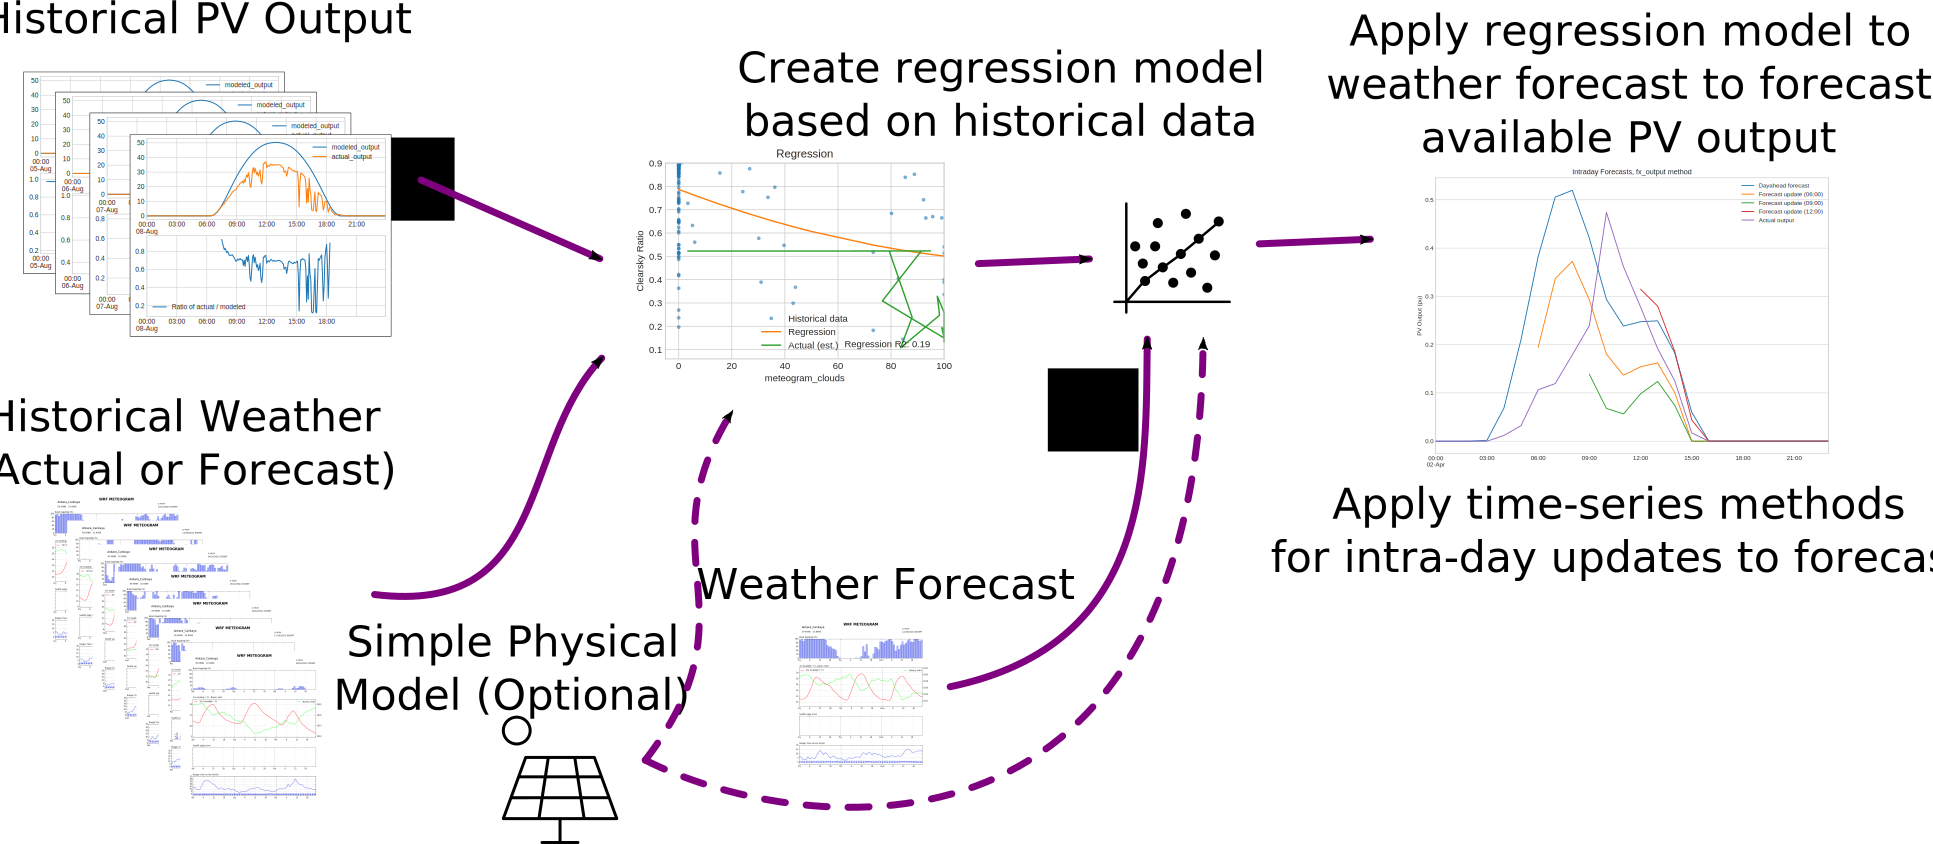
\includegraphics[width=1.0\columnwidth]{PV_forecast_flowchart}
	\caption{Flowchart of Forecasting Method}
	\label{fig:PV_forecast_flowchart}
\end{figure}


\subsection{Day-Ahead Forecasts}
\label{sec:method-day-ahead}

The proposed day-ahead forecasting method combines historical PV output data with historical weather data to infer the relationship between weather and PV output by fitting a simple regression model.
The weather data used is either an estimate of solar irradiance or cloudiness.
\pdfmarkupcomment[color=yellow]{Other weather factors such as temperature are known to influence PV output values,
as well as non-weather factors such as PV aging, dust, and shading.
Because the proposed method uses relatively recent historical PV output data, the longer-term changes related to aging, seasonal temperatures, and dustiness are implicitly tracked as the historical data window moves forward in time.
On the other hand, changes in these factors that are relatively fast compared to the historical time window used will not be accounted for.
Shading may be incorporated to some extent if hourly maximum values from recent history are used to calculate the clear-sky output in cloudiness-based forecasts, however, the available PV dataset did not include any shading of the array, so the effectiveness of this method is addressing shading is not demonstrated.}{Added discussion of other factors affecting PV output as suggested by Reviewer \#1.}

Some pre-processing of the historical data was done prior to  fitting the regression model.
Data from periods of darkness, when output goes to small or negative values, were removed.
This also removed periods when the PV array was covered with snow.

How the regression model was applied depends on the weather data that was used.
If the weather data used represented the incoming solar energy, then the regression was done directly between the weather data and PV output.
For this work, global horizontal irradiance (ghi) was modeled in this way.
A linear model of the form shown in \cref{eqn:ghi-regression-model} was fit to the historical data, where
$P_{PV}$ is the actual or forecast PV output power in per-unit of the array's nominal output rating,
$k_1$ is a linear constant to be fit, and
$GHI$ is actual or forecast global horizontal irradiance.
%
\begin{equation}
	\label{eqn:ghi-regression-model}
	P_{PV} = k_1 \cdot GHI
\end{equation}

On the other hand, weather data, such as cloudiness, that represented the attenuation of incoming solar energy was regressed against the clear-sky ratio for PV output.
Two methods were developed for calculating the clear-sky ratio.
The first method was to roughly model the PV array using data for its geographic position and orientation to obtain modeled clear-sky output.
The second method was to estimate the maximum possible output at each time of day by calculating the maximum observed PV output for each time of day in the historical data window.
This second method had the advantage of not requiring any modeling information about the PV array.
It had the further advantage of naturally incorporating effects of shading of the array during parts of the day due to obstructions.
Since the data set used for this analysis did not include any shading of the array, this last benefit could not be assessed in comparison to other methods.

The formula used to calculate the clear-sky ratio is shown in \cref{eqn:clear-sky-ratio},
where $r_{cs}$ is the clear-sky ratio, $P_{out}$ is the PV output, and $P_{cs}$ is the clear-sky PV output.
In order to provide numerical stability of the clear-sky ratio for periods when the clear-sky output is small, the parameters $\epsilon$ and $r_\epsilon$ were incorporated so that as $P_{cs}$ goes to zero, the clear-sky ratio $r_{cs}$ will approach $r_\epsilon$.
%
\begin{equation}
	\label{eqn:clear-sky-ratio}
	r_{cs} = \frac{P_{out} + r_\epsilon \epsilon}{P_{cs} + \epsilon}
\end{equation}

The regression model was then fit to the transformed data.
A second-degree polynomial model of the form shown in \cref{eqn:cloudiness-regression-model} was used to model the relationship between cloudiness and the clear-sky ratio, where
$r_{cs}$ is the actual or forecast clear-sky ratio,
$k_2$, $k_1$, and $k_0$ are coefficients to be fit, and
$\zeta$ is actual or forecast cloudiness in a range from 0 (no clouds) to 100 (completely cloudy).
%
\begin{equation}
	\label{eqn:cloudiness-regression-model}
	r_{cs} = k_2 \zeta^2 + k_1 \zeta + k_0
\end{equation}

The fit model was then applied to the weather forecast data available for the forecast period.
If applicable, the resulting forecast was then converted from a forecast clear-sky ratio back to PV output using \cref{eqn:clear-sky-ratio}.

\subsection{Intra-day Updates}
\label{sec:method-intraday}

Based on the assumption that updated weather forecasts are in general not obtained throughout the day, the current-day PV output forecast was updated using time-series techniques.
The AR and SARIMAX time-series models are described in time-series modeling/forecasting references\cite{box2015time,korstanje2021}.
Several approaches to intra-day updates were investigated as described in the following paragraphs.

\textit{AR(2) on actual output with exogenous variable:}
An auto-regressive time series model with two lags was applied to the actual clear-sky output ratio with the day-ahead clear-sky output forecast included in the model as an exogenous variable.

\textit{SARIMAX:}
A seasonal auto-regressive integrated moving average model was applied to the actual PV power output with day-ahead output power forecast included in the model as an exogenous variable.
This model is characterized by parameters for the number of auto-regressive (AR) lags $p$, order of differencing (I) $d$, and order of the moving average (MA) $q$, for both the trend and seasonal components.
A variety of parameter combinations was tested against the data, and the best performing model was with AR $p=1$ and MA $q=2$, with the day-ahead PV output power forecast as an exogenous variable, and with no differencing or seasonal components included.

\textit{AR(2) on residual of PV output:}
An auto-regressive time series model with two lags was applied to the residual between actual PV output and the day-ahead forecast PV output. The forecast output of the model was then added as a correction term to the day-ahead PV output forecast for the intra-day period.


\begin{removal}
\pdfmarkupcomment[color=red]{\textit{AR(2) on residual of clear-sky ratio:}
An auto-regressive time series model with two lags was applied to the residual between the actual clear-sky ratio and the day-ahead forecast clear-sky ratio. The forecast output of the model was then added as a correction term to the day-ahead clear-sky ratio forecast for the intra-day period.}{Remove this method from the report to save space. I don't think it adds much.}
\end{removal}

\textit{Scaling:}
The day-ahead forecast for the rest of the day was scaled using the ratio between the actual output in the previous period and the day-ahead forecast for the previous period.

